\documentclass[12pt,reqno]{amsart}
%\documentclass[../Solutions_Introduction_to_Algorithms.tex]{subfiles}
\usepackage{amsmath,amsfonts,amscd,amssymb,epsf,color,enumerate,graphicx,url}
\usepackage{algorithm, algorithmic}
\usepackage{forest, tikz, xcolor}
\usetikzlibrary{matrix, positioning}
\setlength{\oddsidemargin}{-0.2in}%
\setlength{\evensidemargin}{-0.2in}%
\setlength{\textwidth}{6.6in}%
\setlength{\topmargin}{-0.5in}%
 \setlength{\textheight}{9.5in}%
 \definecolor{orange}{rgb}{1,0.5,0}
 \pagestyle{plain}
\linespread{1.3}
\usepackage[small]{caption}
\newcommand{\pa}{\partial}
\newcommand{\va}{\vspace{0.4cm}}
\newcommand{\di}{\displaystyle}
\newcommand{\disp}{\displaystyle}


% turn on \answertrue to show the solution
% turn on \answerfalse to hide the solution
\newif\ifanswer
\answertrue
%\answerfalse



\begin{document}
\noindent {\footnotesize Introduction to Algorithms}\hspace{10.5cm} {\footnotesize Solutions}

\vspace{0.5cm}
\hspace{5.5cm}\textbf{\large Exercises in Section 8.2}
\vspace{0.5cm}

\begin{enumerate}[1.]

\item Using Figure 8.2 as a model, illustrate the operation of \textsc{Counting-Sort} on the array $A = \langle 6, 0, 2, 0, 1, 3, 4, 6, 1, 3, 2 \rangle$.
\vspace{0.5cm}

\ifanswer
\noindent {\bf Solution}

\begin{center}
    \begin{tikzpicture}
        \matrix[matrix of nodes,
                nodes={draw, minimum width=0.7cm, minimum height=0.7cm, anchor=center},
                column sep=0pt, row sep=0pt,
                name=m1] 
        {
            \node[fill=none, draw=none, name=m1-0] {$A$}; &
            \node[fill=pink, name=m1-1] {6}; &
            \node[fill=pink, name=m1-2] {0}; &
            \node[fill=pink, name=m1-3] {2}; &
            \node[fill=pink, name=m1-4] {0}; &
            \node[fill=pink, name=m1-5] {1}; &
            \node[fill=pink, name=m1-6] {3}; &
            \node[fill=pink, name=m1-7] {4}; &
            \node[fill=pink, name=m1-8] {6}; &
            \node[fill=pink, name=m1-9] {1}; &
            \node[fill=pink, name=m1-10] {3}; &
            \node[fill=pink, name=m1-11] {2}; \\
        };
        \node[above=2pt of m1-1] {1};
        \node[above=2pt of m1-2] {2};
        \node[above=2pt of m1-3] {3};
        \node[above=2pt of m1-4] {4};
        \node[above=2pt of m1-5] {5};
        \node[above=2pt of m1-6] {6};
        \node[above=2pt of m1-7] {7};
        \node[above=2pt of m1-8] {8};
        \node[above=2pt of m1-9] {9};
        \node[above=2pt of m1-10] {10};
        \node[above=2pt of m1-11] {11};
    
    
        \matrix[matrix of nodes,
                nodes={draw, minimum width=0.7cm, minimum height=0.7cm, anchor=center},
                column sep=0pt, row sep=0pt,
                below=0.5cm of m1,
                name=m2] 
        {
            \node[fill=none, draw=none, name=m2-0] {$C$}; &
            \node[fill=pink, name=m2-1] {2}; &
            \node[fill=pink, name=m2-2] {2}; &
            \node[fill=pink, name=m2-3] {2}; &
            \node[fill=pink, name=m2-4] {2}; &
            \node[fill=pink, name=m2-5] {1}; &
            \node[fill=pink, name=m2-6] {0}; &
            \node[fill=pink, name=m2-7] {2}; &
            \node[fill=none, draw=none, name=m2-8] {~}; &
            \node[fill=none, draw=none, name=m2-9] {~}; &
            \node[fill=none, draw=none, name=m2-10] {~}; &
            \node[fill=none, draw=none, name=m2-11] {~}; \\
        };
        \node[above=2pt of m2-1] {0};
        \node[above=2pt of m2-2] {1};
        \node[above=2pt of m2-3] {2};
        \node[above=2pt of m2-4] {3};
        \node[above=2pt of m2-5] {4};
        \node[above=2pt of m2-6] {5};
        \node[above=2pt of m2-7] {6};
    \end{tikzpicture}\\
    (i)\\
    \vspace{1cm}
    \begin{tikzpicture}
        \matrix[matrix of nodes,
                nodes={draw, minimum width=0.7cm, minimum height=0.7cm, anchor=center},
                column sep=0pt, row sep=0pt,
                name=m2] 
        {
            \node[fill=none, draw=none, name=m2-0] {$C$}; &
            \node[fill=pink, name=m2-1] {2}; &
            \node[fill=pink, name=m2-2] {4}; &
            \node[fill=pink, name=m2-3] {6}; &
            \node[fill=pink, name=m2-4] {8}; &
            \node[fill=pink, name=m2-5] {9}; &
            \node[fill=pink, name=m2-6] {9}; &
            \node[fill=pink, name=m2-7] {11}; &
            \node[fill=none, draw=none, name=m2-8] {~}; &
            \node[fill=none, draw=none, name=m2-9] {~}; &
            \node[fill=none, draw=none, name=m2-10] {~}; &
            \node[fill=none, draw=none, name=m2-11] {~}; \\
        };
        \node[above=2pt of m2-1] {0};
        \node[above=2pt of m2-2] {1};
        \node[above=2pt of m2-3] {2};
        \node[above=2pt of m2-4] {3};
        \node[above=2pt of m2-5] {4};
        \node[above=2pt of m2-6] {5};
        \node[above=2pt of m2-7] {6};
    \end{tikzpicture}\\
    (ii)\\
    \vspace{1cm}
    \begin{tikzpicture}
        \matrix[matrix of nodes,
                nodes={draw, minimum width=0.7cm, minimum height=0.7cm, anchor=center},
                column sep=0pt, row sep=0pt,
                name=m1] 
        {
            \node[fill=none, draw=none, name=m1-0] {$B$}; &
            \node[fill=cyan, name=m1-1] {~}; &
            \node[fill=cyan, name=m1-2] {~}; &
            \node[fill=cyan, name=m1-3] {~}; &
            \node[fill=cyan, name=m1-4] {~}; &
            \node[fill=cyan, name=m1-5] {~}; &
            \node[fill=pink, name=m1-6] {2}; &
            \node[fill=cyan, name=m1-7] {~}; &
            \node[fill=cyan, name=m1-8] {~}; &
            \node[fill=cyan, name=m1-9] {~}; &
            \node[fill=cyan, name=m1-10] {~}; &
            \node[fill=cyan, name=m1-11] {~}; \\
        };
        \node[above=2pt of m1-1] {1};
        \node[above=2pt of m1-2] {2};
        \node[above=2pt of m1-3] {3};
        \node[above=2pt of m1-4] {4};
        \node[above=2pt of m1-5] {5};
        \node[above=2pt of m1-6] {6};
        \node[above=2pt of m1-7] {7};
        \node[above=2pt of m1-8] {8};
        \node[above=2pt of m1-9] {9};
        \node[above=2pt of m1-10] {10};
        \node[above=2pt of m1-11] {11};
    
    
        \matrix[matrix of nodes,
                nodes={draw, minimum width=0.7cm, minimum height=0.7cm, anchor=center},
                column sep=0pt, row sep=0pt,
                below=0.5cm of m1,
                name=m2] 
        {
            \node[fill=none, draw=none, name=m2-0] {$C$}; &
            \node[fill=pink, name=m2-1] {2}; &
            \node[fill=pink, name=m2-2] {4}; &
            \node[fill=pink, name=m2-3] {5}; &
            \node[fill=pink, name=m2-4] {8}; &
            \node[fill=pink, name=m2-5] {9}; &
            \node[fill=pink, name=m2-6] {9}; &
            \node[fill=pink, name=m2-7] {11}; &
            \node[fill=none, draw=none, name=m2-8] {~}; &
            \node[fill=none, draw=none, name=m2-9] {~}; &
            \node[fill=none, draw=none, name=m2-10] {~}; &
            \node[fill=none, draw=none, name=m2-11] {~}; \\
        };
        \node[above=2pt of m2-1] {0};
        \node[above=2pt of m2-2] {1};
        \node[above=2pt of m2-3] {2};
        \node[above=2pt of m2-4] {3};
        \node[above=2pt of m2-5] {4};
        \node[above=2pt of m2-6] {5};
        \node[above=2pt of m2-7] {6};
    \end{tikzpicture}\\
    (iii)\\
    \vspace{1cm}
    \begin{tikzpicture}
        \matrix[matrix of nodes,
                nodes={draw, minimum width=0.7cm, minimum height=0.7cm, anchor=center},
                column sep=0pt, row sep=0pt,
                name=m1] 
        {
            \node[fill=none, draw=none, name=m1-0] {$B$}; &
            \node[fill=cyan, name=m1-1] {~}; &
            \node[fill=cyan, name=m1-2] {~}; &
            \node[fill=cyan, name=m1-3] {~}; &
            \node[fill=cyan, name=m1-4] {~}; &
            \node[fill=cyan, name=m1-5] {~}; &
            \node[fill=pink, name=m1-6] {2}; &
            \node[fill=cyan, name=m1-7] {~}; &
            \node[fill=pink, name=m1-8] {3}; &
            \node[fill=cyan, name=m1-9] {~}; &
            \node[fill=cyan, name=m1-10] {~}; &
            \node[fill=cyan, name=m1-11] {~}; \\
        };
        \node[above=2pt of m1-1] {1};
        \node[above=2pt of m1-2] {2};
        \node[above=2pt of m1-3] {3};
        \node[above=2pt of m1-4] {4};
        \node[above=2pt of m1-5] {5};
        \node[above=2pt of m1-6] {6};
        \node[above=2pt of m1-7] {7};
        \node[above=2pt of m1-8] {8};
        \node[above=2pt of m1-9] {9};
        \node[above=2pt of m1-10] {10};
        \node[above=2pt of m1-11] {11};
    
    
        \matrix[matrix of nodes,
                nodes={draw, minimum width=0.7cm, minimum height=0.7cm, anchor=center},
                column sep=0pt, row sep=0pt,
                below=0.5cm of m1,
                name=m2] 
        {
            \node[fill=none, draw=none, name=m2-0] {$C$}; &
            \node[fill=pink, name=m2-1] {2}; &
            \node[fill=pink, name=m2-2] {4}; &
            \node[fill=pink, name=m2-3] {5}; &
            \node[fill=pink, name=m2-4] {7}; &
            \node[fill=pink, name=m2-5] {9}; &
            \node[fill=pink, name=m2-6] {9}; &
            \node[fill=pink, name=m2-7] {11}; &
            \node[fill=none, draw=none, name=m2-8] {~}; &
            \node[fill=none, draw=none, name=m2-9] {~}; &
            \node[fill=none, draw=none, name=m2-10] {~}; &
            \node[fill=none, draw=none, name=m2-11] {~}; \\
        };
        \node[above=2pt of m2-1] {0};
        \node[above=2pt of m2-2] {1};
        \node[above=2pt of m2-3] {2};
        \node[above=2pt of m2-4] {3};
        \node[above=2pt of m2-5] {4};
        \node[above=2pt of m2-6] {5};
        \node[above=2pt of m2-7] {6};
    \end{tikzpicture}\\
    (iv)\\
    \vspace{1cm}
    \begin{tikzpicture}
        \matrix[matrix of nodes,
                nodes={draw, minimum width=0.7cm, minimum height=0.7cm, anchor=center},
                column sep=0pt, row sep=0pt,
                name=m1] 
        {
            \node[fill=none, draw=none, name=m1-0] {$B$}; &
            \node[fill=cyan, name=m1-1] {~}; &
            \node[fill=cyan, name=m1-2] {~}; &
            \node[fill=cyan, name=m1-3] {~}; &
            \node[fill=pink, name=m1-4] {1}; &
            \node[fill=cyan, name=m1-5] {~}; &
            \node[fill=pink, name=m1-6] {2}; &
            \node[fill=cyan, name=m1-7] {~}; &
            \node[fill=pink, name=m1-8] {3}; &
            \node[fill=cyan, name=m1-9] {~}; &
            \node[fill=cyan, name=m1-10] {~}; &
            \node[fill=cyan, name=m1-11] {~}; \\
        };
        \node[above=2pt of m1-1] {1};
        \node[above=2pt of m1-2] {2};
        \node[above=2pt of m1-3] {3};
        \node[above=2pt of m1-4] {4};
        \node[above=2pt of m1-5] {5};
        \node[above=2pt of m1-6] {6};
        \node[above=2pt of m1-7] {7};
        \node[above=2pt of m1-8] {8};
        \node[above=2pt of m1-9] {9};
        \node[above=2pt of m1-10] {10};
        \node[above=2pt of m1-11] {11};
    
    
        \matrix[matrix of nodes,
                nodes={draw, minimum width=0.7cm, minimum height=0.7cm, anchor=center},
                column sep=0pt, row sep=0pt,
                below=0.5cm of m1,
                name=m2] 
        {
            \node[fill=none, draw=none, name=m2-0] {$C$}; &
            \node[fill=pink, name=m2-1] {2}; &
            \node[fill=pink, name=m2-2] {3}; &
            \node[fill=pink, name=m2-3] {5}; &
            \node[fill=pink, name=m2-4] {7}; &
            \node[fill=pink, name=m2-5] {9}; &
            \node[fill=pink, name=m2-6] {9}; &
            \node[fill=pink, name=m2-7] {11}; &
            \node[fill=none, draw=none, name=m2-8] {~}; &
            \node[fill=none, draw=none, name=m2-9] {~}; &
            \node[fill=none, draw=none, name=m2-10] {~}; &
            \node[fill=none, draw=none, name=m2-11] {~}; \\
        };
        \node[above=2pt of m2-1] {0};
        \node[above=2pt of m2-2] {1};
        \node[above=2pt of m2-3] {2};
        \node[above=2pt of m2-4] {3};
        \node[above=2pt of m2-5] {4};
        \node[above=2pt of m2-6] {5};
        \node[above=2pt of m2-7] {6};
    \end{tikzpicture}\\
    (v)\\
    \vspace{1cm}
    \begin{tikzpicture}
        \matrix[matrix of nodes,
                nodes={draw, minimum width=0.7cm, minimum height=0.7cm, anchor=center},
                column sep=0pt, row sep=0pt,
                name=m1] 
        {
            \node[fill=none, draw=none, name=m1-0] {$B$}; &
            \node[fill=cyan, name=m1-1] {~}; &
            \node[fill=cyan, name=m1-2] {~}; &
            \node[fill=cyan, name=m1-3] {~}; &
            \node[fill=pink, name=m1-4] {1}; &
            \node[fill=cyan, name=m1-5] {~}; &
            \node[fill=pink, name=m1-6] {2}; &
            \node[fill=cyan, name=m1-7] {~}; &
            \node[fill=pink, name=m1-8] {3}; &
            \node[fill=cyan, name=m1-9] {~}; &
            \node[fill=cyan, name=m1-10] {~}; &
            \node[fill=pink, name=m1-11] {6}; \\
        };
        \node[above=2pt of m1-1] {1};
        \node[above=2pt of m1-2] {2};
        \node[above=2pt of m1-3] {3};
        \node[above=2pt of m1-4] {4};
        \node[above=2pt of m1-5] {5};
        \node[above=2pt of m1-6] {6};
        \node[above=2pt of m1-7] {7};
        \node[above=2pt of m1-8] {8};
        \node[above=2pt of m1-9] {9};
        \node[above=2pt of m1-10] {10};
        \node[above=2pt of m1-11] {11};
    
    
        \matrix[matrix of nodes,
                nodes={draw, minimum width=0.7cm, minimum height=0.7cm, anchor=center},
                column sep=0pt, row sep=0pt,
                below=0.5cm of m1,
                name=m2] 
        {
            \node[fill=none, draw=none, name=m2-0] {$C$}; &
            \node[fill=pink, name=m2-1] {2}; &
            \node[fill=pink, name=m2-2] {3}; &
            \node[fill=pink, name=m2-3] {5}; &
            \node[fill=pink, name=m2-4] {7}; &
            \node[fill=pink, name=m2-5] {9}; &
            \node[fill=pink, name=m2-6] {9}; &
            \node[fill=pink, name=m2-7] {10}; &
            \node[fill=none, draw=none, name=m2-8] {~}; &
            \node[fill=none, draw=none, name=m2-9] {~}; &
            \node[fill=none, draw=none, name=m2-10] {~}; &
            \node[fill=none, draw=none, name=m2-11] {~}; \\
        };
        \node[above=2pt of m2-1] {0};
        \node[above=2pt of m2-2] {1};
        \node[above=2pt of m2-3] {2};
        \node[above=2pt of m2-4] {3};
        \node[above=2pt of m2-5] {4};
        \node[above=2pt of m2-6] {5};
        \node[above=2pt of m2-7] {6};
    \end{tikzpicture}\\
    (vi)\\
    \vspace{1cm}
    \begin{tikzpicture}
        \matrix[matrix of nodes,
                nodes={draw, minimum width=0.7cm, minimum height=0.7cm, anchor=center},
                column sep=0pt, row sep=0pt,
                name=m1] 
        {
            \node[fill=none, draw=none, name=m1-0] {$B$}; &
            \node[fill=cyan, name=m1-1] {~}; &
            \node[fill=cyan, name=m1-2] {~}; &
            \node[fill=cyan, name=m1-3] {~}; &
            \node[fill=pink, name=m1-4] {1}; &
            \node[fill=cyan, name=m1-5] {~}; &
            \node[fill=pink, name=m1-6] {2}; &
            \node[fill=cyan, name=m1-7] {~}; &
            \node[fill=pink, name=m1-8] {3}; &
            \node[fill=pink, name=m1-9] {4}; &
            \node[fill=cyan, name=m1-10] {~}; &
            \node[fill=pink, name=m1-11] {6}; \\
        };
        \node[above=2pt of m1-1] {1};
        \node[above=2pt of m1-2] {2};
        \node[above=2pt of m1-3] {3};
        \node[above=2pt of m1-4] {4};
        \node[above=2pt of m1-5] {5};
        \node[above=2pt of m1-6] {6};
        \node[above=2pt of m1-7] {7};
        \node[above=2pt of m1-8] {8};
        \node[above=2pt of m1-9] {9};
        \node[above=2pt of m1-10] {10};
        \node[above=2pt of m1-11] {11};
    
    
        \matrix[matrix of nodes,
                nodes={draw, minimum width=0.7cm, minimum height=0.7cm, anchor=center},
                column sep=0pt, row sep=0pt,
                below=0.5cm of m1,
                name=m2] 
        {
            \node[fill=none, draw=none, name=m2-0] {$C$}; &
            \node[fill=pink, name=m2-1] {2}; &
            \node[fill=pink, name=m2-2] {3}; &
            \node[fill=pink, name=m2-3] {5}; &
            \node[fill=pink, name=m2-4] {7}; &
            \node[fill=pink, name=m2-5] {8}; &
            \node[fill=pink, name=m2-6] {9}; &
            \node[fill=pink, name=m2-7] {10}; &
            \node[fill=none, draw=none, name=m2-8] {~}; &
            \node[fill=none, draw=none, name=m2-9] {~}; &
            \node[fill=none, draw=none, name=m2-10] {~}; &
            \node[fill=none, draw=none, name=m2-11] {~}; \\
        };
        \node[above=2pt of m2-1] {0};
        \node[above=2pt of m2-2] {1};
        \node[above=2pt of m2-3] {2};
        \node[above=2pt of m2-4] {3};
        \node[above=2pt of m2-5] {4};
        \node[above=2pt of m2-6] {5};
        \node[above=2pt of m2-7] {6};
    \end{tikzpicture}\\
    (vii)\\
    \vspace{1cm}
    \begin{tikzpicture}
        \matrix[matrix of nodes,
                nodes={draw, minimum width=0.7cm, minimum height=0.7cm, anchor=center},
                column sep=0pt, row sep=0pt,
                name=m1] 
        {
            \node[fill=none, draw=none, name=m1-0] {$B$}; &
            \node[fill=cyan, name=m1-1] {~}; &
            \node[fill=cyan, name=m1-2] {~}; &
            \node[fill=cyan, name=m1-3] {~}; &
            \node[fill=pink, name=m1-4] {1}; &
            \node[fill=cyan, name=m1-5] {~}; &
            \node[fill=pink, name=m1-6] {2}; &
            \node[fill=pink, name=m1-7] {3}; &
            \node[fill=pink, name=m1-8] {3}; &
            \node[fill=pink, name=m1-9] {4}; &
            \node[fill=cyan, name=m1-10] {~}; &
            \node[fill=pink, name=m1-11] {6}; \\
        };
        \node[above=2pt of m1-1] {1};
        \node[above=2pt of m1-2] {2};
        \node[above=2pt of m1-3] {3};
        \node[above=2pt of m1-4] {4};
        \node[above=2pt of m1-5] {5};
        \node[above=2pt of m1-6] {6};
        \node[above=2pt of m1-7] {7};
        \node[above=2pt of m1-8] {8};
        \node[above=2pt of m1-9] {9};
        \node[above=2pt of m1-10] {10};
        \node[above=2pt of m1-11] {11};
    
    
        \matrix[matrix of nodes,
                nodes={draw, minimum width=0.7cm, minimum height=0.7cm, anchor=center},
                column sep=0pt, row sep=0pt,
                below=0.5cm of m1,
                name=m2] 
        {
            \node[fill=none, draw=none, name=m2-0] {$C$}; &
            \node[fill=pink, name=m2-1] {2}; &
            \node[fill=pink, name=m2-2] {3}; &
            \node[fill=pink, name=m2-3] {5}; &
            \node[fill=pink, name=m2-4] {6}; &
            \node[fill=pink, name=m2-5] {8}; &
            \node[fill=pink, name=m2-6] {9}; &
            \node[fill=pink, name=m2-7] {10}; &
            \node[fill=none, draw=none, name=m2-8] {~}; &
            \node[fill=none, draw=none, name=m2-9] {~}; &
            \node[fill=none, draw=none, name=m2-10] {~}; &
            \node[fill=none, draw=none, name=m2-11] {~}; \\
        };
        \node[above=2pt of m2-1] {0};
        \node[above=2pt of m2-2] {1};
        \node[above=2pt of m2-3] {2};
        \node[above=2pt of m2-4] {3};
        \node[above=2pt of m2-5] {4};
        \node[above=2pt of m2-6] {5};
        \node[above=2pt of m2-7] {6};
    \end{tikzpicture}\\
    (viii)\\
    \vspace{1cm}
    \begin{tikzpicture}
        \matrix[matrix of nodes,
                nodes={draw, minimum width=0.7cm, minimum height=0.7cm, anchor=center},
                column sep=0pt, row sep=0pt,
                name=m1] 
        {
            \node[fill=none, draw=none, name=m1-0] {$B$}; &
            \node[fill=cyan, name=m1-1] {~}; &
            \node[fill=cyan, name=m1-2] {~}; &
            \node[fill=pink, name=m1-3] {1}; &
            \node[fill=pink, name=m1-4] {1}; &
            \node[fill=cyan, name=m1-5] {~}; &
            \node[fill=pink, name=m1-6] {2}; &
            \node[fill=pink, name=m1-7] {3}; &
            \node[fill=pink, name=m1-8] {3}; &
            \node[fill=pink, name=m1-9] {4}; &
            \node[fill=cyan, name=m1-10] {~}; &
            \node[fill=pink, name=m1-11] {6}; \\
        };
        \node[above=2pt of m1-1] {1};
        \node[above=2pt of m1-2] {2};
        \node[above=2pt of m1-3] {3};
        \node[above=2pt of m1-4] {4};
        \node[above=2pt of m1-5] {5};
        \node[above=2pt of m1-6] {6};
        \node[above=2pt of m1-7] {7};
        \node[above=2pt of m1-8] {8};
        \node[above=2pt of m1-9] {9};
        \node[above=2pt of m1-10] {10};
        \node[above=2pt of m1-11] {11};
    
    
        \matrix[matrix of nodes,
                nodes={draw, minimum width=0.7cm, minimum height=0.7cm, anchor=center},
                column sep=0pt, row sep=0pt,
                below=0.5cm of m1,
                name=m2] 
        {
            \node[fill=none, draw=none, name=m2-0] {$C$}; &
            \node[fill=pink, name=m2-1] {2}; &
            \node[fill=pink, name=m2-2] {2}; &
            \node[fill=pink, name=m2-3] {5}; &
            \node[fill=pink, name=m2-4] {6}; &
            \node[fill=pink, name=m2-5] {8}; &
            \node[fill=pink, name=m2-6] {9}; &
            \node[fill=pink, name=m2-7] {10}; &
            \node[fill=none, draw=none, name=m2-8] {~}; &
            \node[fill=none, draw=none, name=m2-9] {~}; &
            \node[fill=none, draw=none, name=m2-10] {~}; &
            \node[fill=none, draw=none, name=m2-11] {~}; \\
        };
        \node[above=2pt of m2-1] {0};
        \node[above=2pt of m2-2] {1};
        \node[above=2pt of m2-3] {2};
        \node[above=2pt of m2-4] {3};
        \node[above=2pt of m2-5] {4};
        \node[above=2pt of m2-6] {5};
        \node[above=2pt of m2-7] {6};
    \end{tikzpicture}\\
    (ix)\\
    \vspace{1cm}
    \begin{tikzpicture}
        \matrix[matrix of nodes,
                nodes={draw, minimum width=0.7cm, minimum height=0.7cm, anchor=center},
                column sep=0pt, row sep=0pt,
                name=m1] 
        {
            \node[fill=none, draw=none, name=m1-0] {$B$}; &
            \node[fill=cyan, name=m1-1] {~}; &
            \node[fill=pink, name=m1-2] {0}; &
            \node[fill=pink, name=m1-3] {1}; &
            \node[fill=pink, name=m1-4] {1}; &
            \node[fill=cyan, name=m1-5] {~}; &
            \node[fill=pink, name=m1-6] {2}; &
            \node[fill=pink, name=m1-7] {3}; &
            \node[fill=pink, name=m1-8] {3}; &
            \node[fill=pink, name=m1-9] {4}; &
            \node[fill=cyan, name=m1-10] {~}; &
            \node[fill=pink, name=m1-11] {6}; \\
        };
        \node[above=2pt of m1-1] {1};
        \node[above=2pt of m1-2] {2};
        \node[above=2pt of m1-3] {3};
        \node[above=2pt of m1-4] {4};
        \node[above=2pt of m1-5] {5};
        \node[above=2pt of m1-6] {6};
        \node[above=2pt of m1-7] {7};
        \node[above=2pt of m1-8] {8};
        \node[above=2pt of m1-9] {9};
        \node[above=2pt of m1-10] {10};
        \node[above=2pt of m1-11] {11};
    
    
        \matrix[matrix of nodes,
                nodes={draw, minimum width=0.7cm, minimum height=0.7cm, anchor=center},
                column sep=0pt, row sep=0pt,
                below=0.5cm of m1,
                name=m2] 
        {
            \node[fill=none, draw=none, name=m2-0] {$C$}; &
            \node[fill=pink, name=m2-1] {1}; &
            \node[fill=pink, name=m2-2] {2}; &
            \node[fill=pink, name=m2-3] {5}; &
            \node[fill=pink, name=m2-4] {6}; &
            \node[fill=pink, name=m2-5] {8}; &
            \node[fill=pink, name=m2-6] {9}; &
            \node[fill=pink, name=m2-7] {10}; &
            \node[fill=none, draw=none, name=m2-8] {~}; &
            \node[fill=none, draw=none, name=m2-9] {~}; &
            \node[fill=none, draw=none, name=m2-10] {~}; &
            \node[fill=none, draw=none, name=m2-11] {~}; \\
        };
        \node[above=2pt of m2-1] {0};
        \node[above=2pt of m2-2] {1};
        \node[above=2pt of m2-3] {2};
        \node[above=2pt of m2-4] {3};
        \node[above=2pt of m2-5] {4};
        \node[above=2pt of m2-6] {5};
        \node[above=2pt of m2-7] {6};
    \end{tikzpicture}\\
    (x)\\
    \vspace{1cm}
    \begin{tikzpicture}
        \matrix[matrix of nodes,
                nodes={draw, minimum width=0.7cm, minimum height=0.7cm, anchor=center},
                column sep=0pt, row sep=0pt,
                name=m1] 
        {
            \node[fill=none, draw=none, name=m1-0] {$B$}; &
            \node[fill=cyan, name=m1-1] {~}; &
            \node[fill=pink, name=m1-2] {0}; &
            \node[fill=pink, name=m1-3] {1}; &
            \node[fill=pink, name=m1-4] {1}; &
            \node[fill=pink, name=m1-5] {2}; &
            \node[fill=pink, name=m1-6] {2}; &
            \node[fill=pink, name=m1-7] {3}; &
            \node[fill=pink, name=m1-8] {3}; &
            \node[fill=pink, name=m1-9] {4}; &
            \node[fill=cyan, name=m1-10] {~}; &
            \node[fill=pink, name=m1-11] {6}; \\
        };
        \node[above=2pt of m1-1] {1};
        \node[above=2pt of m1-2] {2};
        \node[above=2pt of m1-3] {3};
        \node[above=2pt of m1-4] {4};
        \node[above=2pt of m1-5] {5};
        \node[above=2pt of m1-6] {6};
        \node[above=2pt of m1-7] {7};
        \node[above=2pt of m1-8] {8};
        \node[above=2pt of m1-9] {9};
        \node[above=2pt of m1-10] {10};
        \node[above=2pt of m1-11] {11};
    
    
        \matrix[matrix of nodes,
                nodes={draw, minimum width=0.7cm, minimum height=0.7cm, anchor=center},
                column sep=0pt, row sep=0pt,
                below=0.5cm of m1,
                name=m2] 
        {
            \node[fill=none, draw=none, name=m2-0] {$C$}; &
            \node[fill=pink, name=m2-1] {1}; &
            \node[fill=pink, name=m2-2] {2}; &
            \node[fill=pink, name=m2-3] {4}; &
            \node[fill=pink, name=m2-4] {6}; &
            \node[fill=pink, name=m2-5] {8}; &
            \node[fill=pink, name=m2-6] {9}; &
            \node[fill=pink, name=m2-7] {10}; &
            \node[fill=none, draw=none, name=m2-8] {~}; &
            \node[fill=none, draw=none, name=m2-9] {~}; &
            \node[fill=none, draw=none, name=m2-10] {~}; &
            \node[fill=none, draw=none, name=m2-11] {~}; \\
        };
        \node[above=2pt of m2-1] {0};
        \node[above=2pt of m2-2] {1};
        \node[above=2pt of m2-3] {2};
        \node[above=2pt of m2-4] {3};
        \node[above=2pt of m2-5] {4};
        \node[above=2pt of m2-6] {5};
        \node[above=2pt of m2-7] {6};
    \end{tikzpicture}\\
    (xi)\\
    \vspace{1cm}
    \begin{tikzpicture}
        \matrix[matrix of nodes,
                nodes={draw, minimum width=0.7cm, minimum height=0.7cm, anchor=center},
                column sep=0pt, row sep=0pt,
                name=m1] 
        {
            \node[fill=none, draw=none, name=m1-0] {$B$}; &
            \node[fill=pink, name=m1-1] {0}; &
            \node[fill=pink, name=m1-2] {0}; &
            \node[fill=pink, name=m1-3] {1}; &
            \node[fill=pink, name=m1-4] {1}; &
            \node[fill=pink, name=m1-5] {2}; &
            \node[fill=pink, name=m1-6] {2}; &
            \node[fill=pink, name=m1-7] {3}; &
            \node[fill=pink, name=m1-8] {3}; &
            \node[fill=pink, name=m1-9] {4}; &
            \node[fill=cyan, name=m1-10] {~}; &
            \node[fill=pink, name=m1-11] {6}; \\
        };
        \node[above=2pt of m1-1] {1};
        \node[above=2pt of m1-2] {2};
        \node[above=2pt of m1-3] {3};
        \node[above=2pt of m1-4] {4};
        \node[above=2pt of m1-5] {5};
        \node[above=2pt of m1-6] {6};
        \node[above=2pt of m1-7] {7};
        \node[above=2pt of m1-8] {8};
        \node[above=2pt of m1-9] {9};
        \node[above=2pt of m1-10] {10};
        \node[above=2pt of m1-11] {11};
    
    
        \matrix[matrix of nodes,
                nodes={draw, minimum width=0.7cm, minimum height=0.7cm, anchor=center},
                column sep=0pt, row sep=0pt,
                below=0.5cm of m1,
                name=m2] 
        {
            \node[fill=none, draw=none, name=m2-0] {$C$}; &
            \node[fill=pink, name=m2-1] {0}; &
            \node[fill=pink, name=m2-2] {2}; &
            \node[fill=pink, name=m2-3] {4}; &
            \node[fill=pink, name=m2-4] {6}; &
            \node[fill=pink, name=m2-5] {8}; &
            \node[fill=pink, name=m2-6] {9}; &
            \node[fill=pink, name=m2-7] {10}; &
            \node[fill=none, draw=none, name=m2-8] {~}; &
            \node[fill=none, draw=none, name=m2-9] {~}; &
            \node[fill=none, draw=none, name=m2-10] {~}; &
            \node[fill=none, draw=none, name=m2-11] {~}; \\
        };
        \node[above=2pt of m2-1] {0};
        \node[above=2pt of m2-2] {1};
        \node[above=2pt of m2-3] {2};
        \node[above=2pt of m2-4] {3};
        \node[above=2pt of m2-5] {4};
        \node[above=2pt of m2-6] {5};
        \node[above=2pt of m2-7] {6};
    \end{tikzpicture}\\
    (xii)\\
    \vspace{1cm}
    \begin{tikzpicture}
        \matrix[matrix of nodes,
                nodes={draw, minimum width=0.7cm, minimum height=0.7cm, anchor=center},
                column sep=0pt, row sep=0pt,
                name=m1] 
        {
            \node[fill=none, draw=none, name=m1-0] {$B$}; &
            \node[fill=pink, name=m1-1] {0}; &
            \node[fill=pink, name=m1-2] {0}; &
            \node[fill=pink, name=m1-3] {1}; &
            \node[fill=pink, name=m1-4] {1}; &
            \node[fill=pink, name=m1-5] {2}; &
            \node[fill=pink, name=m1-6] {2}; &
            \node[fill=pink, name=m1-7] {3}; &
            \node[fill=pink, name=m1-8] {3}; &
            \node[fill=pink, name=m1-9] {4}; &
            \node[fill=pink, name=m1-10] {6}; &
            \node[fill=pink, name=m1-11] {6}; \\
        };
        \node[above=2pt of m1-1] {1};
        \node[above=2pt of m1-2] {2};
        \node[above=2pt of m1-3] {3};
        \node[above=2pt of m1-4] {4};
        \node[above=2pt of m1-5] {5};
        \node[above=2pt of m1-6] {6};
        \node[above=2pt of m1-7] {7};
        \node[above=2pt of m1-8] {8};
        \node[above=2pt of m1-9] {9};
        \node[above=2pt of m1-10] {10};
        \node[above=2pt of m1-11] {11};
    \end{tikzpicture}\\
    (xiii)\\
\end{center}
\vspace{1cm}



\item Prove that \textsc{Counting-Sort} is stable.
\vspace{0.5cm}

\ifanswer
\noindent {\bf Solution}

\noindent It suffices to show that for any two equal elements, say $A[i] = A[j] = x$, where $i < j$, the index of $A[i]$ is less than $A[j]$. Note that the loop in line 11-13 applies downward iterations, that is, $A[j]$ is iterated before $A[i]$. Line 13 then guarantees $C[x]$, the index, is lower for $A[i]$ than it was for $A[j]$. \qed
\vspace{1cm}



\item Suppose that we were to rewrite the \textbf{for} loop header in line 11 of the \textsc{Counting-Sort} as \begin{center} \textbf{for} $j = 1$ \textbf{to} $n$ \end{center} Show that the algorithm still works property, but that it is not stable. Then rewrite the pseudocode for counting sort so that elements with the same value are written into the output array in order of increasing index and the algorithm is stable.
\vspace{0.5cm}

\ifanswer
\noindent {\bf Solution}

\noindent With forward iteration, the sorting algorithm still works, because the order of elements in the original array $A$ does not affect the correctness of the output (you can even iterate $A$ in any weird order). However, for two elements $A[i]$ and $A[j]$ with the same value, where $i < j$, $A[i]$ will appear later than $A[j]$ with similar reason as in the previous question. So, the new algorithm is not stable. Below shows an updated algorithm that is stable:
\begin{algorithm}
    \caption{\textsc{Forward-Counting-Sort}$(A, n, k)$}
    \begin{algorithmic}[1]
        \STATE let $B[1:n]$ and $C[0:k]$ be new arrays
        \FOR{$i = 0$ to $k$}
            \STATE $C[i] = 0$
        \ENDFOR
        \FOR{$j = 1$ to $n$}
            \STATE $C[A[j]] = C[A[j]] + 1$
        \ENDFOR
        \FOR{$i = 1$ to $k$}
            \STATE $C[i] = C[i] + C[i - 1]$
        \ENDFOR
        \FOR{$i = k$ downto $1$}
            \STATE $C[i] = C[i - 1] + 1$
        \ENDFOR
        \STATE $C[0] = 1$
        \FOR{$j = 1$ to $n$}
            \STATE $B[C[A[j]]] = A[j]$
            \STATE $C[A[j]] = C[A[j]] + 1$
        \ENDFOR
        \RETURN $B$
    \end{algorithmic}
\end{algorithm}
\vspace{1cm}



\item Prove the following loop invariant for \textsc{Counting-Sort}: At the start of each iteration of the \textbf{for} loop of lines 11-13, the last element in $A$ with value $i$ that has not yet been copied into $B$ belongs in $B[C[i]]$.
\vspace{0.5cm}

\ifanswer
\noindent {\bf Solution}

\begin{itemize}
    \item Initialization: Before the first iteration, $C[i]$ is the number of elements with value less than or equal to $i$. Therefore, the last element with value $i$ should be located to $B[C[i]]$, the last slot for value $i$.
    \item Maintenance: Suppose we are at index $j$ and $A[j] = i$, and $A[j]$ belongs to $B[C[i]]$ in this iteration. In line 13, $C[i]$ is reduced by 1, therefore, $B[C[i]]$ should exactly contain the next element with value $i$. \qed
\end{itemize}
\vspace{1cm}



\item Suppose that the array being sorted contains only integers in the range $0$ to $k$ and that there are no satellite data to move with those keys. Modify counting sort to use just the arrays $A$ and $C$, putting the sorted result back into array $A$ instead of into a new array $B$.
\vspace{0.5cm}

\ifanswer
\noindent {\bf Solution}

\begin{algorithm}
    \caption{\textsc{Modified-Counting-Sort}$(A, n, k)$}
    \begin{algorithmic}[1]
        \STATE let $C[0:k]$ be a new array
        \FOR{$i = 0$ to $k$}
            \STATE $C[i] = 0$
        \ENDFOR
        \FOR{$j = 1$ to $n$}
            \STATE $C[A[j]] = C[A[j]] + 1$
        \ENDFOR
        \STATE $index = 1$
        \FOR{$i = 0$ to $k$}
            \FOR{$j = 1$ to $C[i]$}
                \STATE $A[index] = i$
                \STATE $index = index + 1$
            \ENDFOR
        \ENDFOR
        \RETURN $A$
    \end{algorithmic}
\end{algorithm}
\vspace{1cm}



\item Describe an algorithm that, given $n$ integers in the range $0$ to $k$, preprocesses its input and then answers any query about how many of the $n$ integers fall into a range $[a:b]$ in $O(1)$ time. Your algorithm should use $\Theta(n + k)$ preprocessing time.
\vspace{0.5cm}

\ifanswer
\noindent {\bf Solution}

\noindent Given an interval $[a:b]$, the key idea is to find the number of integers that are larger than or equal to $a$, and the number of integers that are smaller than or equal to $b$. Basic set theory then tells us the answer equals the sum of these two numbers minus $n$. The preprocessing algorithm:
\begin{algorithm}
    \caption{\textsc{Preprocess-Integers}$(A, n, k)$}
    \begin{algorithmic}[1]
        \STATE let $C[0:k]$ and $D[0:k]$ be new arrays
        \FOR{$i = 0$ to $k$}
            \STATE $C[i] = 0$
            \STATE $D[i] = 0$
        \ENDFOR
        \FOR{$j = 1$ to $n$}
            \STATE $C[A[j]] = C[A[j]] + 1$
            \STATE $D[A[j]] = D[A[j]] + 1$
        \ENDFOR
        \FOR{$i = 1$ to $k$}
            \STATE $C[i] = C[i] + C[i - 1]$
        \ENDFOR
        \FOR{$i = k - 1$ downto $0$}
            \STATE $D[i] = D[i] + D[i + 1]$
        \ENDFOR
        \RETURN $C, D$
    \end{algorithmic}
\end{algorithm}

\noindent Once we have the arrays $C$ and $D$, the number of integers falling in $[a:b]$ is equal to $$C[a] + D[b] - n,$$ finishing in $O(1)$ time.
\vspace{1cm}


\item Counting sort can also work efficiently if the input values have fractional parts, but the number of digits in the fractional part is small. Suppose that you are given $n$ number in the range $0$ to $k$, each with at most $d$ decimal (base $10$) digits to the right of the decimal point. Modify counting sort to run in $\Theta(n + {10}^dk)$ time.
\vspace{0.5cm}

\ifanswer
\noindent {\bf Solution}

\noindent The key idea is to multiply each decimal number by ${10}^d$, therefore we are dealing with $n$ integers in the range $0$ to ${10}^dk$. For this reason, we will call the original counting sort algorithm in the modified algorithm:
\begin{algorithm}
    \caption{\textsc{Modified-Counting-Sort}$(A, n, k, d)$}
    \begin{algorithmic}[1]
        \STATE let $B[1:n]$ be a new array
        \FOR{$i = 0$ to $n$}
            \STATE $B[i] = {10}^d * A[i]$
        \ENDFOR
        \RETURN \textsc{Counting-Sort}$(B, n, {10}^d * k)$
    \end{algorithmic}
\end{algorithm}
\vspace{1cm}



\end{enumerate}

\end{document}



